\documentclass[twoside]{book}

% Packages required by doxygen
\usepackage{fixltx2e}
\usepackage{calc}
\usepackage{doxygen}
\usepackage[export]{adjustbox} % also loads graphicx
\usepackage{graphicx}
\usepackage[utf8]{inputenc}
\usepackage{makeidx}
\usepackage{multicol}
\usepackage{multirow}
\PassOptionsToPackage{warn}{textcomp}
\usepackage{textcomp}
\usepackage[nointegrals]{wasysym}
\usepackage[table]{xcolor}

% Font selection
\usepackage[T1]{fontenc}
\usepackage[scaled=.90]{helvet}
\usepackage{courier}
\usepackage{amssymb}
\usepackage{sectsty}
\renewcommand{\familydefault}{\sfdefault}
\allsectionsfont{%
  \fontseries{bc}\selectfont%
  \color{darkgray}%
}
\renewcommand{\DoxyLabelFont}{%
  \fontseries{bc}\selectfont%
  \color{darkgray}%
}
\newcommand{\+}{\discretionary{\mbox{\scriptsize$\hookleftarrow$}}{}{}}

% Page & text layout
\usepackage{geometry}
\geometry{%
  a4paper,%
  top=2.5cm,%
  bottom=2.5cm,%
  left=2.5cm,%
  right=2.5cm%
}
\tolerance=750
\hfuzz=15pt
\hbadness=750
\setlength{\emergencystretch}{15pt}
\setlength{\parindent}{0cm}
\setlength{\parskip}{3ex plus 2ex minus 2ex}
\makeatletter
\renewcommand{\paragraph}{%
  \@startsection{paragraph}{4}{0ex}{-1.0ex}{1.0ex}{%
    \normalfont\normalsize\bfseries\SS@parafont%
  }%
}
\renewcommand{\subparagraph}{%
  \@startsection{subparagraph}{5}{0ex}{-1.0ex}{1.0ex}{%
    \normalfont\normalsize\bfseries\SS@subparafont%
  }%
}
\makeatother

% Headers & footers
\usepackage{fancyhdr}
\pagestyle{fancyplain}
\fancyhead[LE]{\fancyplain{}{\bfseries\thepage}}
\fancyhead[CE]{\fancyplain{}{}}
\fancyhead[RE]{\fancyplain{}{\bfseries\leftmark}}
\fancyhead[LO]{\fancyplain{}{\bfseries\rightmark}}
\fancyhead[CO]{\fancyplain{}{}}
\fancyhead[RO]{\fancyplain{}{\bfseries\thepage}}
\fancyfoot[LE]{\fancyplain{}{}}
\fancyfoot[CE]{\fancyplain{}{}}
\fancyfoot[RE]{\fancyplain{}{\bfseries\scriptsize Generated by Doxygen }}
\fancyfoot[LO]{\fancyplain{}{\bfseries\scriptsize Generated by Doxygen }}
\fancyfoot[CO]{\fancyplain{}{}}
\fancyfoot[RO]{\fancyplain{}{}}
\renewcommand{\footrulewidth}{0.4pt}
\renewcommand{\chaptermark}[1]{%
  \markboth{#1}{}%
}
\renewcommand{\sectionmark}[1]{%
  \markright{\thesection\ #1}%
}

% Indices & bibliography
\usepackage{natbib}
\usepackage[titles]{tocloft}
\setcounter{tocdepth}{3}
\setcounter{secnumdepth}{5}
\makeindex

% Hyperlinks (required, but should be loaded last)
\usepackage{ifpdf}
\ifpdf
  \usepackage[pdftex,pagebackref=true]{hyperref}
\else
  \usepackage[ps2pdf,pagebackref=true]{hyperref}
\fi
\hypersetup{%
  colorlinks=true,%
  linkcolor=blue,%
  citecolor=blue,%
  unicode%
}

% Custom commands
\newcommand{\clearemptydoublepage}{%
  \newpage{\pagestyle{empty}\cleardoublepage}%
}

\usepackage{caption}
\captionsetup{labelsep=space,justification=centering,font={bf},singlelinecheck=off,skip=4pt,position=top}

%===== C O N T E N T S =====

\begin{document}

% Titlepage & ToC
\hypersetup{pageanchor=false,
             bookmarksnumbered=true,
             pdfencoding=unicode
            }
\pagenumbering{alph}
\begin{titlepage}
\vspace*{7cm}
\begin{center}%
{\Large T\+DD Group 4 P\+ID Controller }\\
\vspace*{1cm}
{\large Generated by Doxygen 1.8.13}\\
\end{center}
\end{titlepage}
\clearemptydoublepage
\pagenumbering{roman}
\tableofcontents
\clearemptydoublepage
\pagenumbering{arabic}
\hypersetup{pageanchor=true}

%--- Begin generated contents ---
\chapter{Class Index}
\section{Class List}
Here are the classes, structs, unions and interfaces with brief descriptions\+:\begin{DoxyCompactList}
\item\contentsline{section}{\hyperlink{classttd_1_1PID}{ttd\+::\+P\+ID} }{\pageref{classttd_1_1PID}}{}
\end{DoxyCompactList}

\chapter{File Index}
\section{File List}
Here is a list of all documented files with brief descriptions\+:\begin{DoxyCompactList}
\item\contentsline{section}{app/\hyperlink{main_8cpp}{main.\+cpp} \\*This is a the main class for the P\+ID implementation project P\+ID controller implementation for mobile robot }{\pageref{main_8cpp}}{}
\item\contentsline{section}{app/\hyperlink{pid_8cpp}{pid.\+cpp} \\*"Copyright \mbox{[}2019\mbox{]} Markose Jacob, Maitreya Kulkarni }{\pageref{pid_8cpp}}{}
\item\contentsline{section}{include/{\bfseries pid.\+hpp} }{\pageref{pid_8hpp}}{}
\end{DoxyCompactList}

\chapter{Class Documentation}
\hypertarget{classttd_1_1PID}{}\section{ttd\+:\+:P\+ID Class Reference}
\label{classttd_1_1PID}\index{ttd\+::\+P\+ID@{ttd\+::\+P\+ID}}
\subsection*{Public Member Functions}
\begin{DoxyCompactItemize}
\item 
double \hyperlink{classttd_1_1PID_a296c7b460949bb9f9883d9990dc59415}{Compute} ()
\begin{DoxyCompactList}\small\item\em Header files. \end{DoxyCompactList}\item 
double \hyperlink{classttd_1_1PID_a21a0403413a68aa1da98a75257dbde8a}{get\+\_\+kp} ()
\item 
\mbox{\Hypertarget{classttd_1_1PID_aaee3d5cd5e3dce62590c0fc6b554fa07}\label{classttd_1_1PID_aaee3d5cd5e3dce62590c0fc6b554fa07}} 
double {\bfseries get\+\_\+ki} ()
\item 
double \hyperlink{classttd_1_1PID_a84e6add940d84fab262f98a835cdb97a}{get\+\_\+kd} ()
\item 
\mbox{\Hypertarget{classttd_1_1PID_aac6255851baf7e31ddf00bde7439b539}\label{classttd_1_1PID_aac6255851baf7e31ddf00bde7439b539}} 
{\bfseries P\+ID} (double kp=1, double ki=1, double kd=1, double target\+\_\+velocity=10, double actual\+\_\+velocity=5)
\end{DoxyCompactItemize}
\subsection*{Public Attributes}
\begin{DoxyCompactItemize}
\item 
\mbox{\Hypertarget{classttd_1_1PID_a2a3149842acf22de82012477999c861c}\label{classttd_1_1PID_a2a3149842acf22de82012477999c861c}} 
double {\bfseries target\+\_\+velocity\+\_\+}
\item 
\mbox{\Hypertarget{classttd_1_1PID_a4b25b31ff787740f372e2d92f4198b8a}\label{classttd_1_1PID_a4b25b31ff787740f372e2d92f4198b8a}} 
double {\bfseries actual\+\_\+velocity\+\_\+}
\end{DoxyCompactItemize}


\subsection{Member Function Documentation}
\mbox{\Hypertarget{classttd_1_1PID_a296c7b460949bb9f9883d9990dc59415}\label{classttd_1_1PID_a296c7b460949bb9f9883d9990dc59415}} 
\index{ttd\+::\+P\+ID@{ttd\+::\+P\+ID}!Compute@{Compute}}
\index{Compute@{Compute}!ttd\+::\+P\+ID@{ttd\+::\+P\+ID}}
\subsubsection{\texorpdfstring{Compute()}{Compute()}}
{\footnotesize\ttfamily double ttd\+::\+P\+I\+D\+::\+Compute (\begin{DoxyParamCaption}{ }\end{DoxyParamCaption})}



Header files. 

This is the function which computes the pid calculations  nil \begin{DoxyReturn}{Returns}
returns 
\end{DoxyReturn}
\mbox{\Hypertarget{classttd_1_1PID_a84e6add940d84fab262f98a835cdb97a}\label{classttd_1_1PID_a84e6add940d84fab262f98a835cdb97a}} 
\index{ttd\+::\+P\+ID@{ttd\+::\+P\+ID}!get\+\_\+kd@{get\+\_\+kd}}
\index{get\+\_\+kd@{get\+\_\+kd}!ttd\+::\+P\+ID@{ttd\+::\+P\+ID}}
\subsubsection{\texorpdfstring{get\+\_\+kd()}{get\_kd()}}
{\footnotesize\ttfamily double ttd\+::\+P\+I\+D\+::get\+\_\+kd (\begin{DoxyParamCaption}{ }\end{DoxyParamCaption})}

Function to access value of kd \begin{DoxyReturn}{Returns}
value of kd 
\end{DoxyReturn}
Function to access value of ki \begin{DoxyReturn}{Returns}
value of ki
\end{DoxyReturn}
\mbox{\Hypertarget{classttd_1_1PID_a21a0403413a68aa1da98a75257dbde8a}\label{classttd_1_1PID_a21a0403413a68aa1da98a75257dbde8a}} 
\index{ttd\+::\+P\+ID@{ttd\+::\+P\+ID}!get\+\_\+kp@{get\+\_\+kp}}
\index{get\+\_\+kp@{get\+\_\+kp}!ttd\+::\+P\+ID@{ttd\+::\+P\+ID}}
\subsubsection{\texorpdfstring{get\+\_\+kp()}{get\_kp()}}
{\footnotesize\ttfamily double ttd\+::\+P\+I\+D\+::get\+\_\+kp (\begin{DoxyParamCaption}{ }\end{DoxyParamCaption})}

Function to access value of kp \begin{DoxyReturn}{Returns}
value of kp 
\end{DoxyReturn}


The documentation for this class was generated from the following files\+:\begin{DoxyCompactItemize}
\item 
include/pid.\+hpp\item 
app/\hyperlink{pid_8cpp}{pid.\+cpp}\end{DoxyCompactItemize}

\chapter{File Documentation}
\hypertarget{main_8cpp}{}\section{app/main.cpp File Reference}
\label{main_8cpp}\index{app/main.\+cpp@{app/main.\+cpp}}


This is a the main class for the P\+ID implementation project P\+ID controller implementation for mobile robot.  


{\ttfamily \#include $<$iostream$>$}\newline
{\ttfamily \#include \char`\"{}../include/pid.\+hpp\char`\"{}}\newline
Include dependency graph for main.\+cpp\+:\nopagebreak
\begin{figure}[H]
\begin{center}
\leavevmode
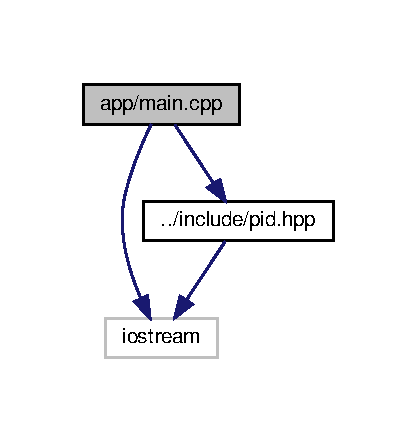
\includegraphics[width=200pt]{main_8cpp__incl}
\end{center}
\end{figure}
\subsection*{Functions}
\begin{DoxyCompactItemize}
\item 
\mbox{\Hypertarget{main_8cpp_ae66f6b31b5ad750f1fe042a706a4e3d4}\label{main_8cpp_ae66f6b31b5ad750f1fe042a706a4e3d4}} 
int \hyperlink{main_8cpp_ae66f6b31b5ad750f1fe042a706a4e3d4}{main} ()
\begin{DoxyCompactList}\small\item\em Main compute function for P\+ID Controller. \end{DoxyCompactList}\end{DoxyCompactItemize}


\subsection{Detailed Description}
This is a the main class for the P\+ID implementation project P\+ID controller implementation for mobile robot. 

\begin{DoxyAuthor}{Author}
Markose Jacob, Maitreya Kulkarni 
\end{DoxyAuthor}
\begin{DoxyDate}{Date}
26 Spetember 2019 
\end{DoxyDate}
\begin{DoxyCopyright}{Copyright}
\mbox{[}2021\mbox{]} $<$Maitreya Kulkarni , Markose Jacob$>$ 
\end{DoxyCopyright}

\hypertarget{pid_8cpp}{}\section{app/pid.cpp File Reference}
\label{pid_8cpp}\index{app/pid.\+cpp@{app/pid.\+cpp}}


"Copyright \mbox{[}2019\mbox{]} Markose Jacob, Maitreya Kulkarni  


{\ttfamily \#include \char`\"{}../include/pid.\+hpp\char`\"{}}\newline
{\ttfamily \#include $<$iostream$>$}\newline
Include dependency graph for pid.\+cpp\+:\nopagebreak
\begin{figure}[H]
\begin{center}
\leavevmode
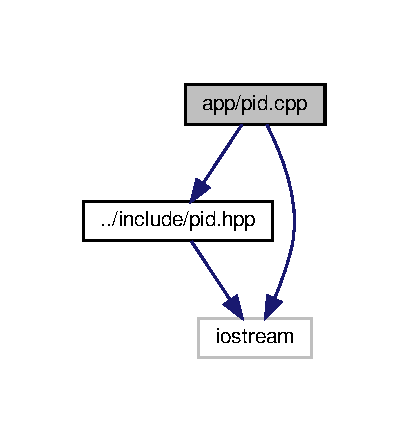
\includegraphics[width=196pt]{pid_8cpp__incl}
\end{center}
\end{figure}


\subsection{Detailed Description}
"Copyright \mbox{[}2019\mbox{]} Markose Jacob, Maitreya Kulkarni 

\begin{DoxyAuthor}{Author}
Maitreya Kulkarni (Driver), Markose Jacob (Navigator) 
\end{DoxyAuthor}
\begin{DoxyDate}{Date}
2 October 2021 
\end{DoxyDate}
\begin{DoxyCopyright}{Copyright}
2021 Maitreya Kulkarni, Markose Jacob This is a class for a P\+ID controller 
\end{DoxyCopyright}

%--- End generated contents ---

% Index
\backmatter
\newpage
\phantomsection
\clearemptydoublepage
\addcontentsline{toc}{chapter}{Index}
\printindex

\end{document}
